\section{Appendix B}
\section{B 1 - Informed consent form}
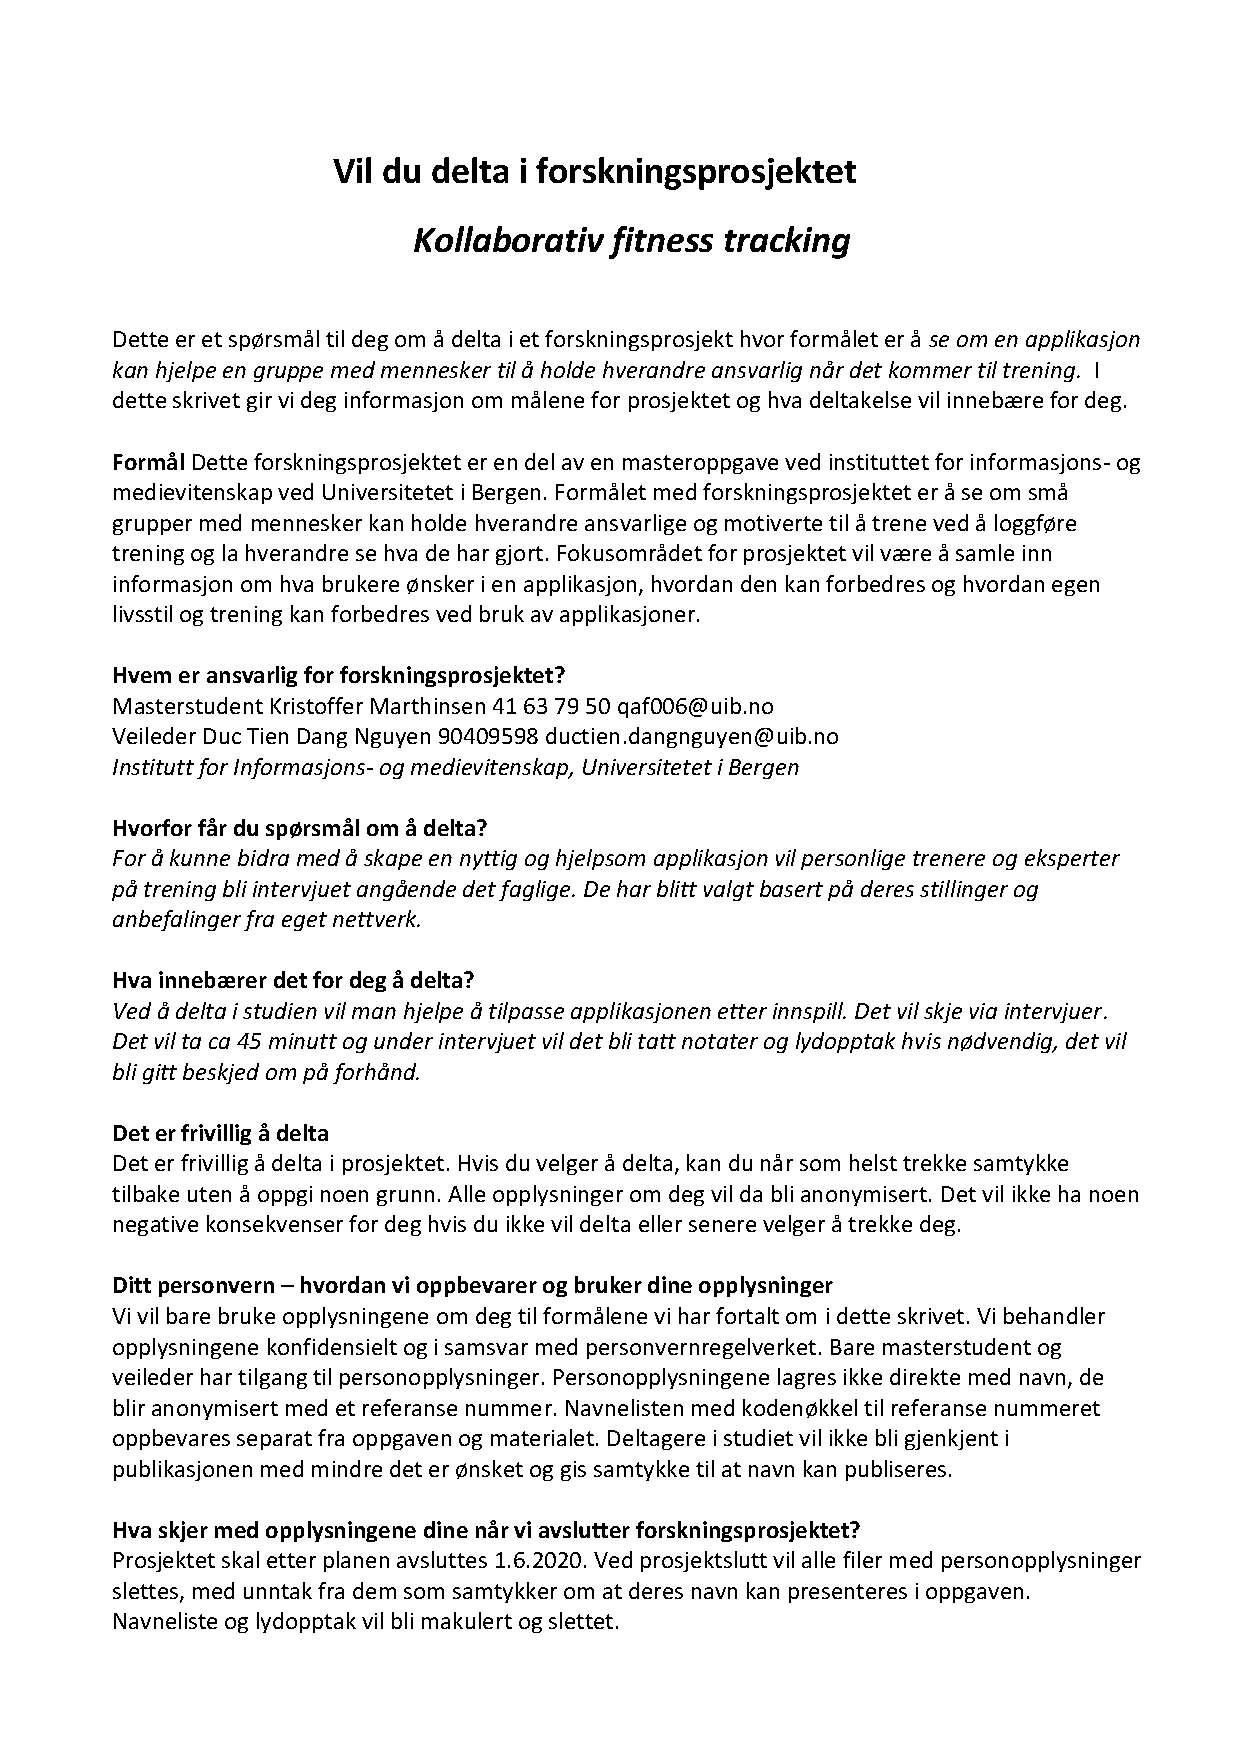
\includepdf[pages=-]{pdfAppendix/InformasjonsSkriv.pdf}

\section{B 2 - Interview guide for experts}
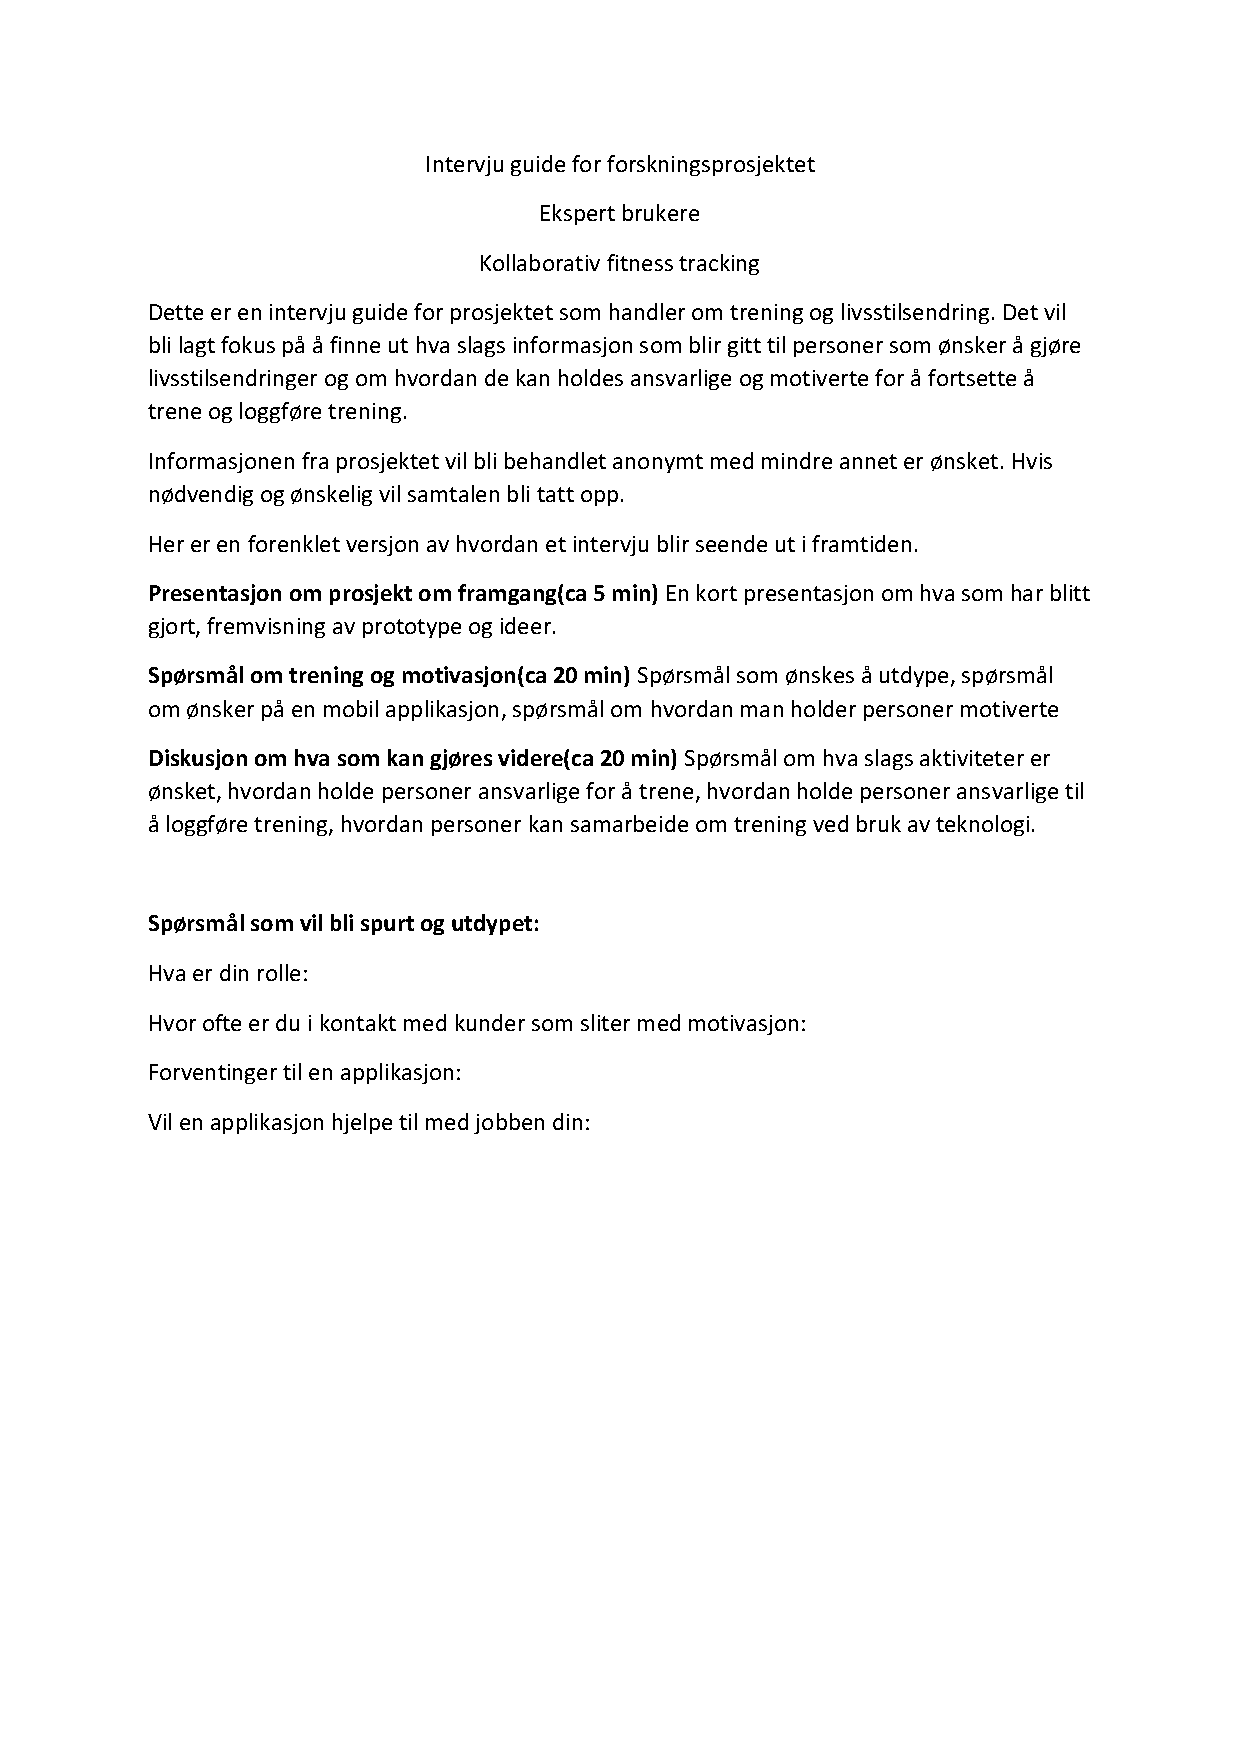
\includepdf[pages=-]{pdfAppendix/expertGuide.pdf}

\section{B 3 - Interview guide for users}
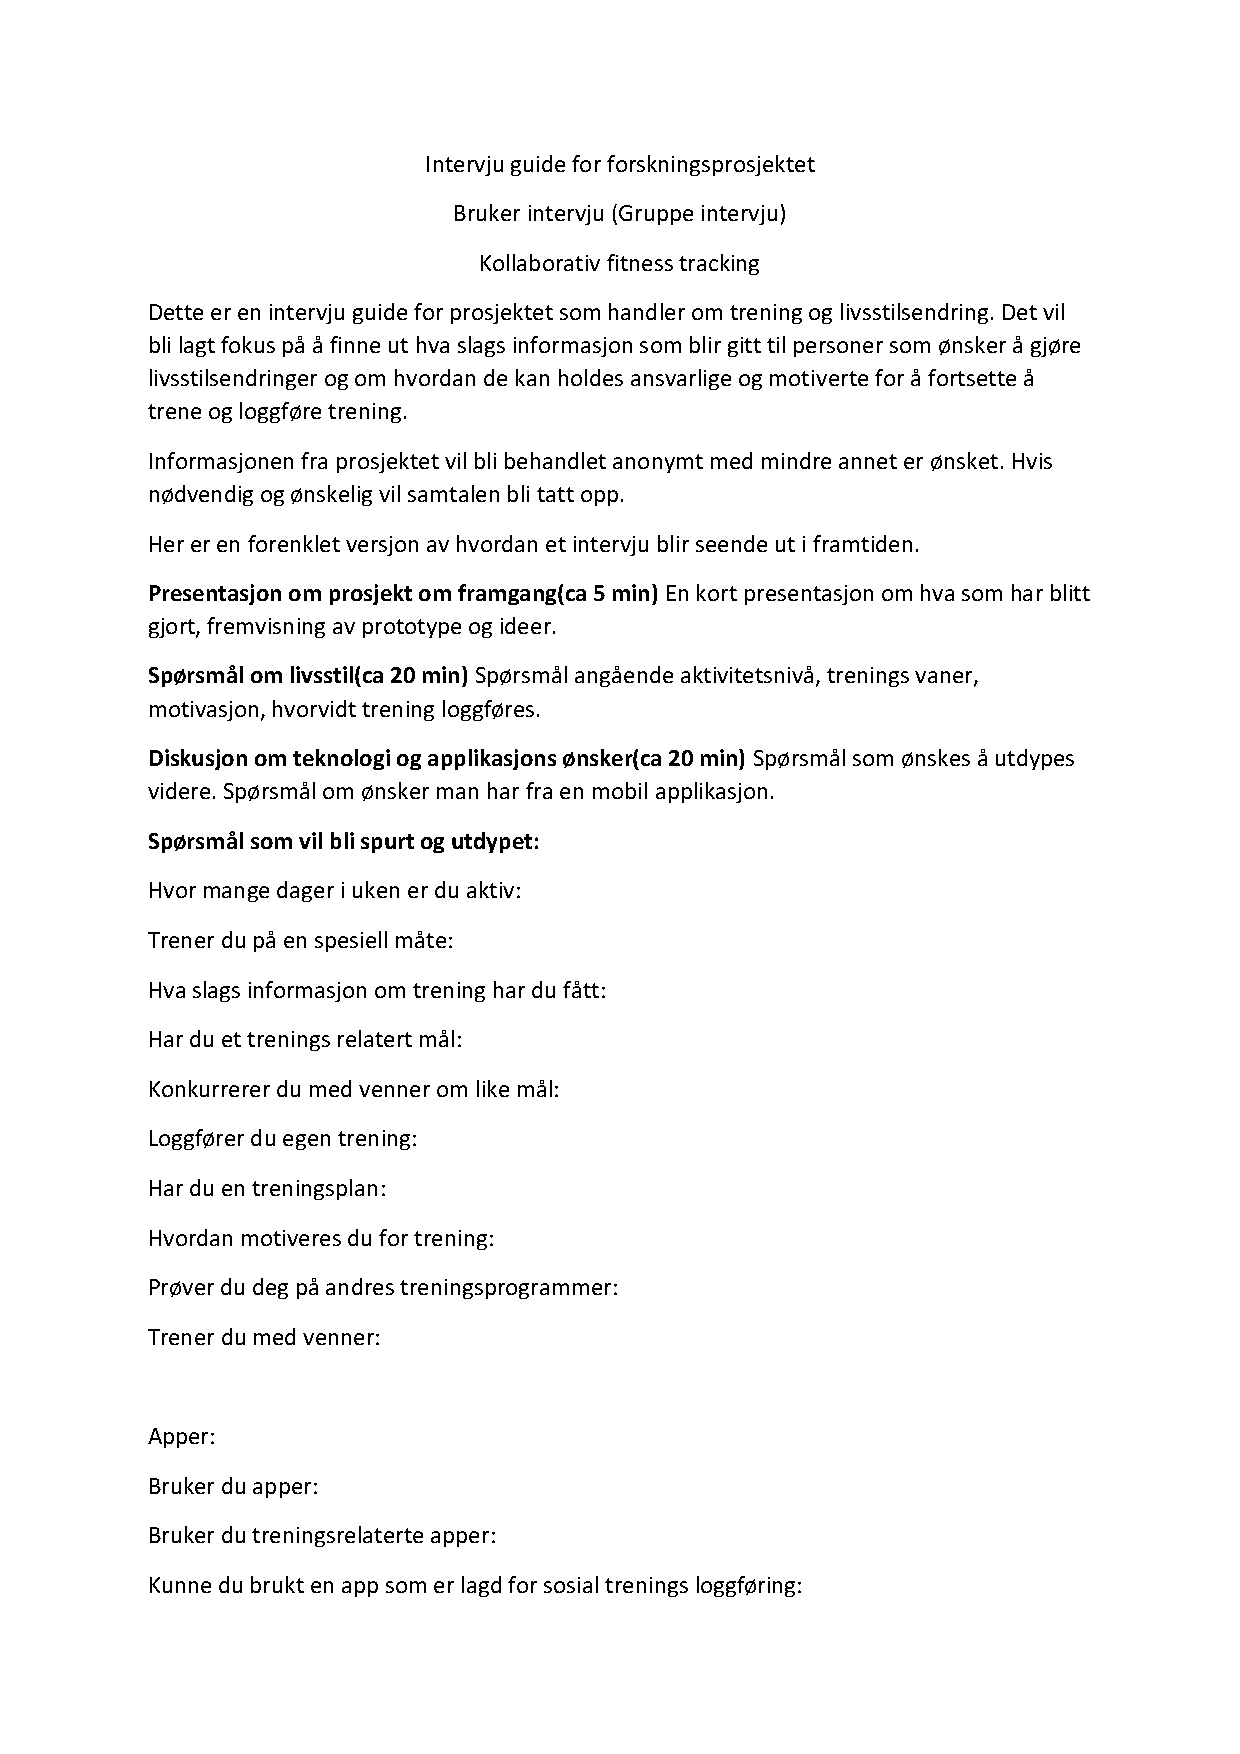
\includepdf[pages=-]{pdfAppendix/groupGuide.pdf}
\section{B 4 - System usability scale form}
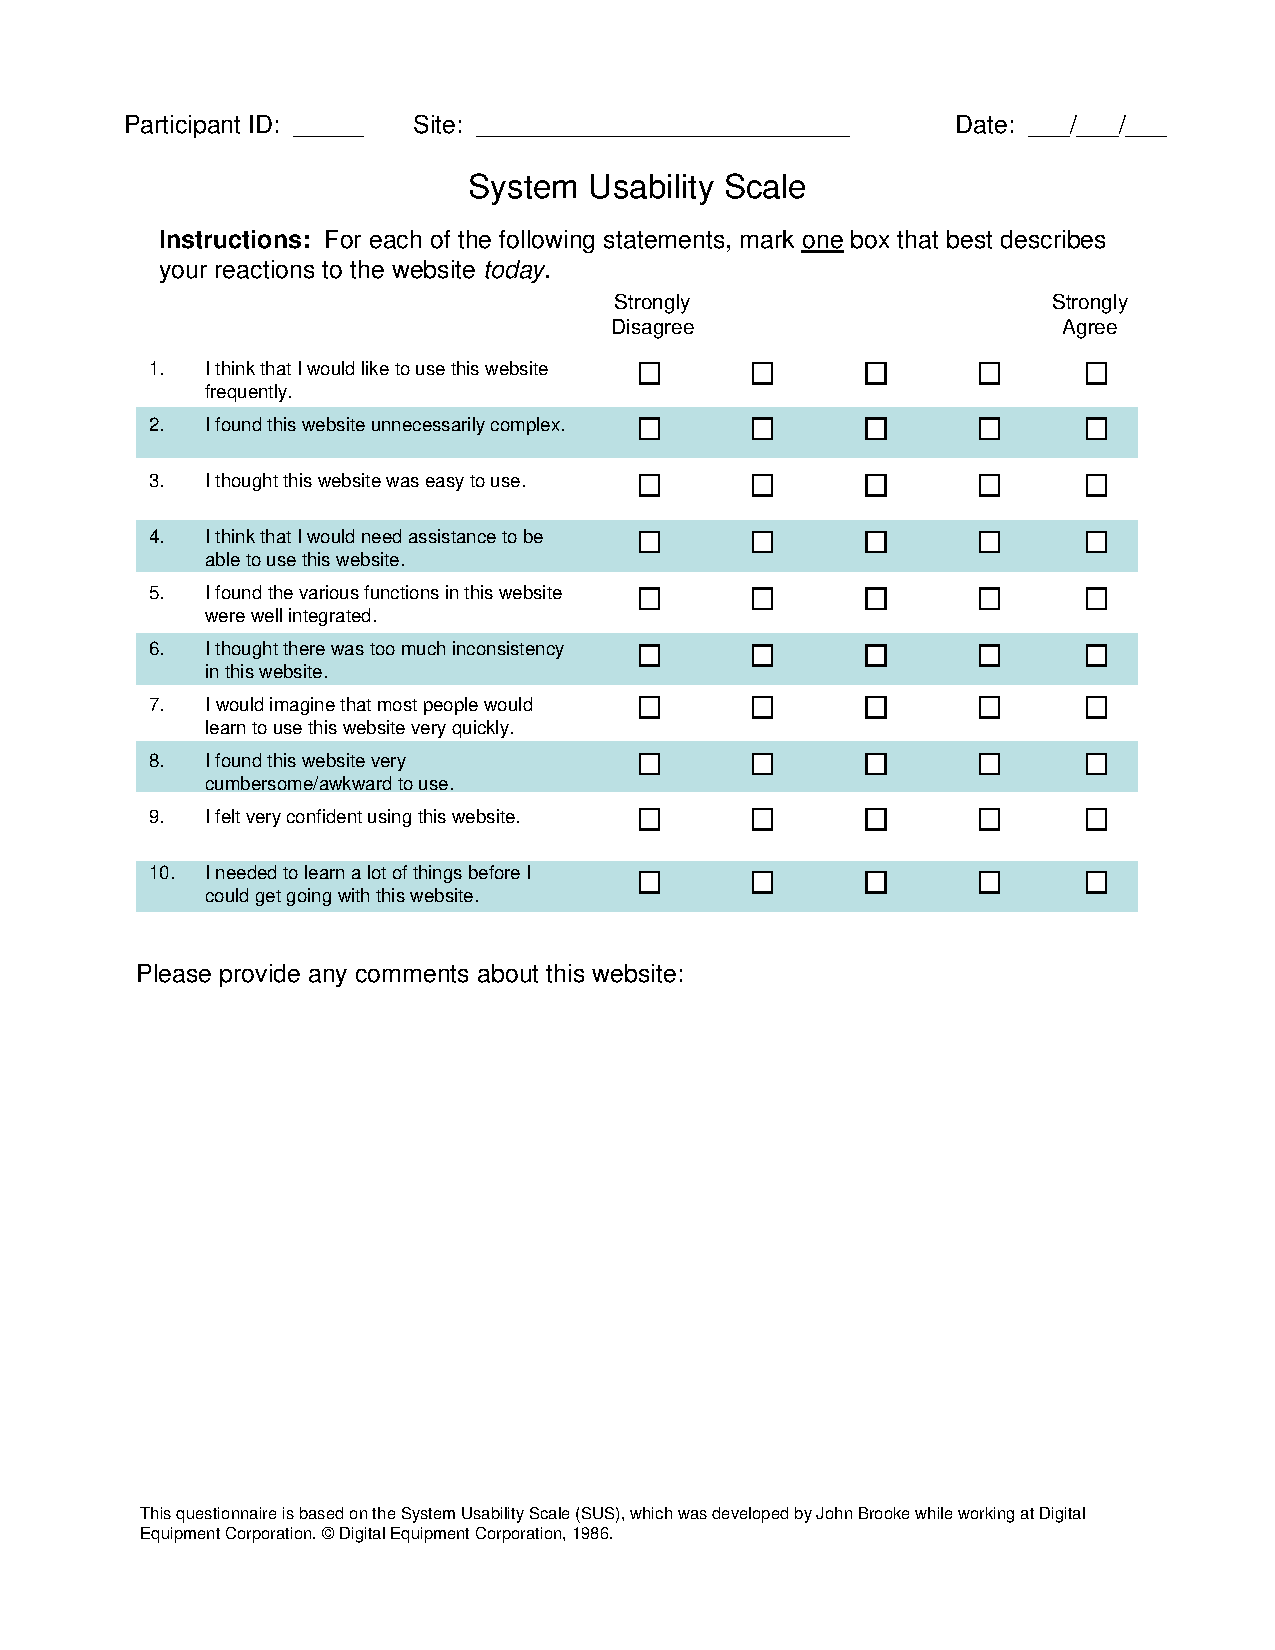
\includepdf[pages=-]{pdfAppendix/SUS.pdf}

\section{Development tools}
\subsection{Proto.io}
Proto.io is an application prototyping platform \cite{proto} that can can simulate everything an app can do. That includes interactive touch gestures, screen transitions and animations. It allows users to create realistic, shareable prototypes that work as a real app should and experience their prototype on the actual device.
\subsection{ReactJS}
ReactJS is a javascript library for building user interfaces \cite{react}. It is a flexible and efficient front end javascript library for building user interfaces\cite{react2}. ReactJS is developed by Facebook and is used by a variety of websites and applications. 

\subsection{Google forms}
Google Forms is a tool that allows collecting information from users via a personalized survey or quiz. The information is then collected and automatically connected to a spreadsheet\cite{forms}. Google forms was used to create a survey that was shared on social media, which helped gather valuable information.
\subsection{Atom}
Atom is the text-editor that was used to code in for this project. With atom it is possible to import packages, have multiple panes, manage packages and helps you write code faster with a smart and flexible autocomplete \cite{atom}.   
\subsection{Github}
Github provides software development version control using git. It provides access control and several collaboration features such as bug tracking, feature requests, task management, and wikis for every project \cite{github} . 